\documentclass[12pt]{article}

\usepackage[margin=1in]{geometry}
\usepackage{parskip}
\usepackage{amsmath}
\usepackage[backend=biber, style=alphabetic, sorting=ynt]{biblatex}
\usepackage{graphicx}
\usepackage{wrapfig}
\usepackage{float}
\usepackage{caption}
\usepackage{hyperref}

\graphicspath{{./images/}}

\begin{document}

\title{Applying State Space Control Theory to the Pole Balancing Problem}
\author{Brendon Matusch}
\date{November 2018}
\maketitle

\section{Introduction}

\subsection{The Pole Balancing Problem}

One of the most famous problems in control theory is the \textit{pole balancing problem}, also known as \textit{cart pole}. The basic idea of the problem is as follows:
\begin{itemize}
    \item A movable cart sits on a straight, finite-length track.
    \item A pole (light, relative to the cart) is anchored to the cart with a hinge.
    \item A motor is attached to the cart; it can accelerate the cart to the left or right.
    \item The goal is to prevent the pole from falling over, while also keeping the cart near the center of the track.
\end{itemize}

\begin{figure}[h]
    \centering
    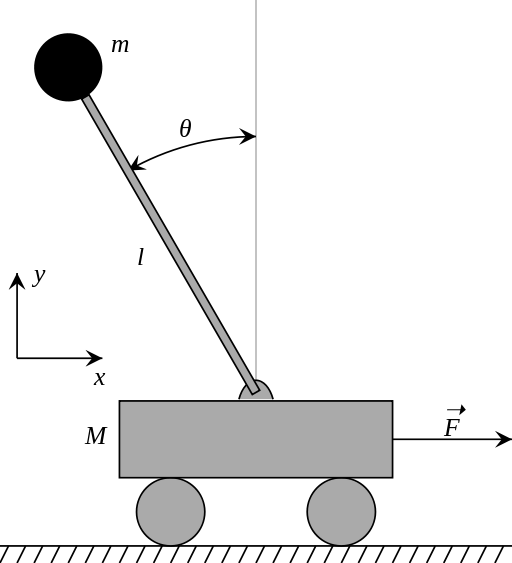
\includegraphics[width=180pt]{cartpole}
    \caption{\label{cartpole} A diagram of the pole balancing problem.}
\end{figure}

This problem is quite clearly not trivial. If the pole starts to fall to the right, one must accelerate the cart to the right to prevent it from falling over. However, that also results in the cart moving away from the center. Thus, to successfully optimize both the angle and the position, one must gradually adjust the angle by applying small forces while the cart moves.

\subsection{Control Algorithms}

The most common classical solution to this kind of problem is the PID (proportional, integral, and derivative) closed control loop.

\end{document}